
%***********************************************************************
% PLEASE LEAVE THIS PART UNCHANGED
%***********************************************************************

\documentclass[twoside]{report}
\usepackage{iwsm}
\usepackage{graphicx}
\usepackage{amsmath, amssymb}
\usepackage{booktabs}

% Please do not specify any new definitions, any new commands,
% and do not specify any style parameters.
% The preamble of the document should be left unchanged.

\begin{document}

%***********************************************************************
% PLEASE INSERT YOUR CONTENT FROM HERE
%***********************************************************************

% Title and running title to be used as left header:
%\title{Exploring LD decay with quantiles -- a case study}
\title{Quantifying LD decay by quantile regression -- a case study} 
\titlerunning{Quantiles for LD decay}

% Authors and running list of authors to be used as right header:
\author{Sabine K. Schnabel\inst{1}, Federico Torretta\inst{2} and Matthias Westhues \inst{3}}
\authorrunning{Schnabel et al.}    %% use \authorrunning{Surname 1} if only 1 author
                                    %% use \authorrunning{Surname 1 and Surname2} if two authors
                                    %% use \authorrunning{Surname 1 et al.} if more than two authors

% Institutes of all authors
% Include city and country of each institute, do not include the full address.
\institute{Biometris, Wageningen University and Research Centre,
The Netherlands \and Universit\`a di Palermo, Italy \and Universit\"at Hohenheim, Germany}

% E-mail of presenting author for correspondence
\email{sabine.schnabel@wur.nl}

% Brief abstract of the paper:
\abstract{Through recent developments in genotyping (e.g. of plant 
populations) more information on genetic markers become available. In order 
to perform powerful genome-wide 
association studies (GWAS) it is important to analyse linkage disequilibrium (LD) through 
pairwise comparisons of genetic markers. Large numbers of these markers pose new problems 
in terms of analysis and visualization. In a case study for Maize we 
explore and quantify LD decay using monotone quantile regression.}

% Keywords (at most 5):
\keywords{Quantile regression; smoothing; monotonicity; linkage; LD decay}

% Produce the title:
\maketitle

%***********************************************************************

% Sections and subsections (do not use lower levels):


\section{Introduction and Motivation}
Genome-wide association studies have emerged as a great tool for the 
localization of QTLs (quantitative trait loci) in plant and animal breeding programs.
However, a crucial requirement to powerful GWAS is the investigation of the genetic 
relatedness (kinship matrix) (Astle and Balding, 2009). 
For an appropriate kinship matrix, insight into LD between 
genetic markers is necessary. This matrix is best based on a set of independent markers 
(Listgarten et al., 2012).
To find such a set of suitable markers (e.g. single nucleotide polymorphism -- SNP) we need 
to explore LD decay over the whole genome . LD is commonly measured in terms of 
the squared Pearson correlation $R^2$ between pairs of genetic
markers (Hill and Robertson, 1968). As an example, we are using data from chromosome 1 of a Maize 
population consisting of 123 European Dent inbred lines and 114 European Flint inbred lines
(Fischer et al., 2008). Figure~\ref{SchnabelTorrettaWesthues:fig1}~(A) shows an LD decay plot 
for this part of the genome. 

\section{Analysis and Application}

Chromosome 1 of the above described 
Maize genome has almost 5000 markers, resulting in more than 
12 million pairwise comparisons 
	between two markers on the same chromosome. Visualization of these large data sets is 
	challenging. We used a scatterplot smoother (Eilers and Goeman, 2004) for depicting
	global LD decay on chromosome 1 (length $\approx$ 300 Mbp (Mega base pairs))   
	in Figure~\ref{SchnabelTorrettaWesthues:fig1}~(A). As mentioned above, the most 
	common measure for LD decay is the squared Pearson correlation $R^2$. In order to improve the 
	quality of the fit as well as the visualization, we advocate to use $\sqrt{|R|}$ instead. Further 
	investigation concerning this transformation will be reported elsewhere. 
	In our case it is of interest to examine what happens to 
	LD decay on a smaller scale. Therefore we investigate local LD decay in subsequent 
	overlapping sliding windows of 2.5 Mbp width and fit a set of quantile curves to each of these 
	sections on the whole plot.  
	We use quantile 
	regression with a monotonicity constraint,
	$\mu_{\tau}=s_{\tau}(d)$, where $\mu_\tau$ is the quantile function at 
	percentile $\tau$, $d$ is the SNP distance between pairs of markers and 
	$s_{\tau}(\cdot)$ is a smooth and unknown function (Muggeo et al., 2013; Bollaerts et al., 2006). 
	We choose $B-$splines for a smooth functional form. By imposing 
	$b_k<b_{k-1}$, with $b_{k}$ coefficient of the $B_k$-th spline, 
	a monotone decreasing curve is ensured (that is 
	in line with the underlying biological assumptions). This analysis can be done for any quantile 
	of interest. In Figure~\ref{SchnabelTorrettaWesthues:fig1}~(B) quantile curves for 
	$\tau={0.25,0.5,0.75}$ are 
	plotted as well as a threshold in terms of LD decay (on the initial scale 
	of $R^2$=0.1, therefore here $\sqrt[4]{0.1}$). For the exploration of local LD decay 
	we might be interested in the distance $\Delta_{0.5}$ from 
	which onwards the LD decay is falling beneath the threshold. This can be interpreted as the
	average distance within this window from which onwards two marker loci are considered to be 
	independent of each other. Such two markers could, for example, be selected for the computation
	of a kinship matrix. In the example, local 
		LD decay in terms of median distance at threshold $\sqrt[4]{0.1}$ is 249666 bp. 
	On Chromosome 1 of this population we have about 1000 sliding windows
	 of 2.5 Mbp width with an 
	average of 2000 points falling into one window. The distances 
	$\Delta_{\tau}$ for all sliding windows are collected and plotted 
	in Figure~\ref{SchnabelTorrettaWesthues:fig1}~(C) 
	at the respective center of the window. We collect these data for  
	$\tau$ values that are of interest. While these data points are an interesting result as
	such to quantify local LD decay, it is hard to judge by eye the relationship that is plotted in 
	Figure~\ref{SchnabelTorrettaWesthues:fig1}~(C). 
	Therefore we used $P-$splines to fit a smooth curve to these results as 
	displayed by the curve in Figure~\ref{SchnabelTorrettaWesthues:fig1}~(D). 
	For our example, we detect a bi-modal form of the 
	relationship. The black line in the graph indicates the so-called centromere. 
	We have reason to believe that the left mode is around the centromere.   
	However, this bi-modal phenomenon could not be observed for 
	all of the 10 chromosomes in this data set.   

\section{Conclusion and Discussion}
This is a case study of how to explore and quantify local LD decay patterns in maize. We are using
quantile regression with monotonicity constraints for a first summary of the LD decay. 
On top of that we are applying $P-$splines to smoothen the median local LD decay. These curves 
are easier to interpret and to inspect for the collaborating biologists. 

While the presented steps are a good tool to quantify local LD decay, they have also been 
	instrumental in identifying problems with the underlying genotypic 
	data that have previously been 
	overlooked. In this sense they can serve as a diagnostic tool. 
	On the one hand we discovered sliding windows with low sample sizes which suggests 
	undercoverage in certain distances in LD decay. 
	While fitting the smooth curves in Figure~\ref{SchnabelTorrettaWesthues:fig1}~(D), we 
	observed a noticeable clustering 
	in terms of correlation values in some of the subsets of the data. This phenomenon was unknown 
	to date in this data set and has lead to adjustments to subsequent data analyses. 
	
More results from this case study will be reported elsewhere.

\begin{figure}[bt!]\centering
	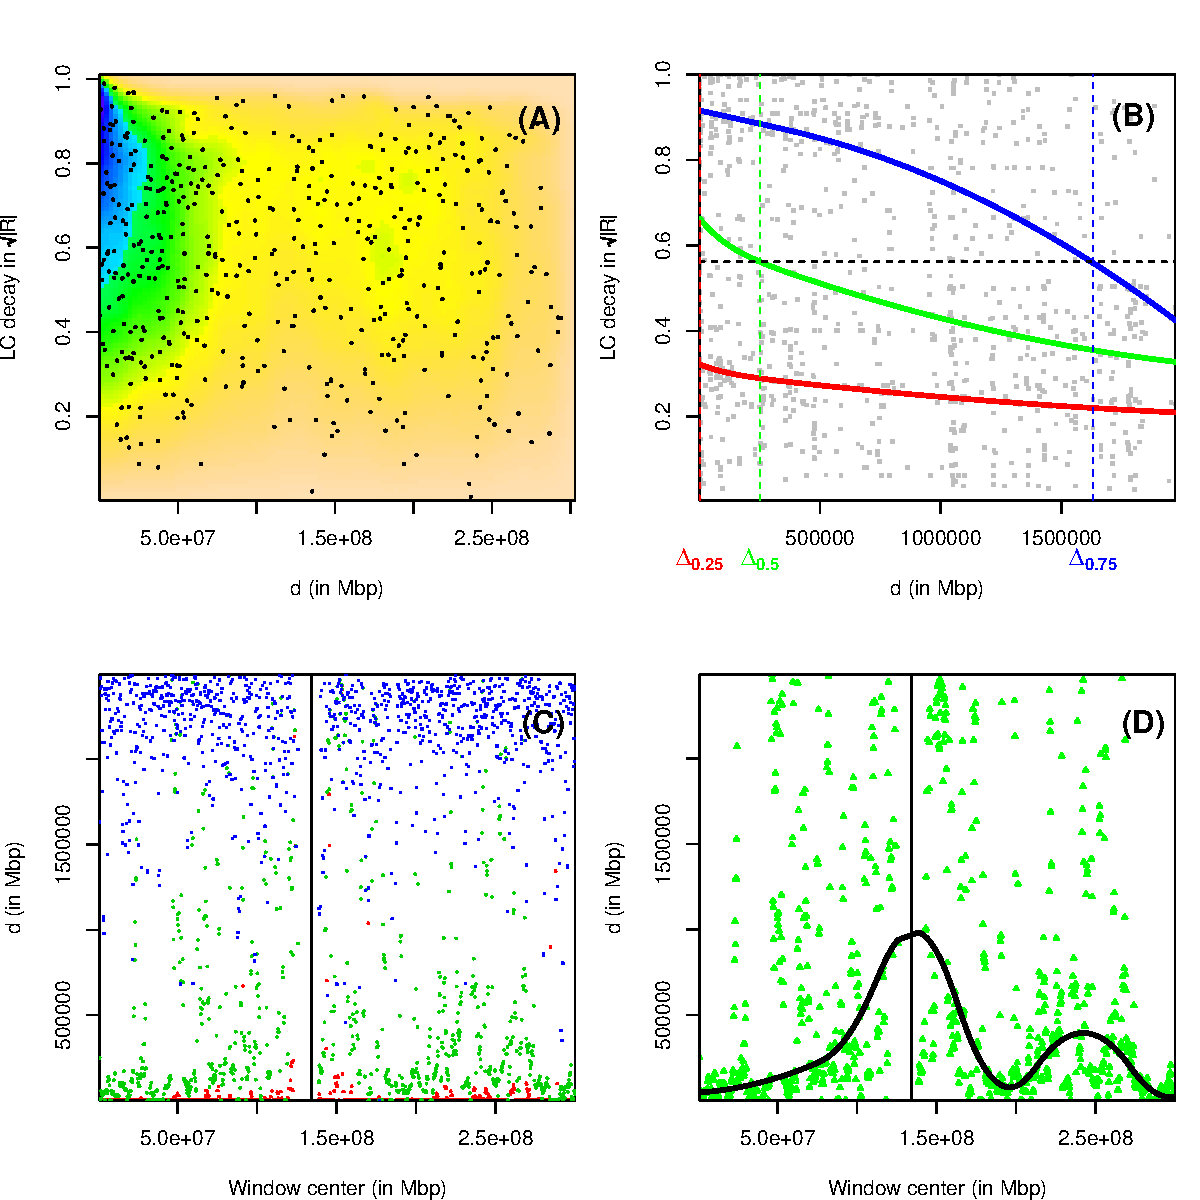
\includegraphics[width=0.8\textwidth]{Figure1_final.pdf}
\caption{\label{SchnabelTorrettaWesthues:fig1} (A) Plot of LD decay for Chromosome 1 
using \texttt{scattersmooth}. 
(B) Sample of 
data with threshold $R^2$=0.1 and $\Delta_{0.25,0.5,0.75}$ indication. 
(C) Collection of $\Delta_{0.25,0.5,0.75}$ in 
Red/Green/Blue for Chromosome 1 at the center of the sliding window with indication of the centromere. 
(D) Smooth fit to $\Delta_{0.5}$.}
\end{figure}

%***********************************************************************

% Acknowledgments, if needed:
\acknowledgments{This case study was performed while the second and third author were 
visiting at Biometris at Wageningen University and Research Centre in winter 2014/2015. We are indebted to the group of Prof. Dr. Ruedi Fries, from Technische Universit\"at M\"unchen, for the SNP genotyping of the parental lines, which was funded by the German Federal Ministry of Education and Research (BMBF)  within the AgroClustEr “Synbreed—Synergistic plant and animal breeding” (FKZ:0315528d).}

%***********************************************************************


\references
\begin{description}
\item[Astle, W. and Balding, D.J.] (2009).
		Population Structure and Cryptic Relatedness in Genetic Association Studies.
		{\it Statistical Science}, {\bf 24}, 451\,--\,471
\item[Bollaerts, K., Eilers, P.H.C. and M. Aerts] (2006). Quantile regression with monotonicity restrictions using P-splines and the L1-norm. {\it Statistical Modelling}, {\bf 6}, 189\,--\,207 
\item[Bush, W.S. and Moore, J.H.] (2012).
		Chapter 11: Genome-wide association studies.
		{\it PLOS Computational Biology}, {\bf 8}, 1\,--\,11

\item[Eilers, P.H.C. and Goeman, J.J.] (2004).
	Enhancing scatterplots with smoothed density.
	{\it Bioinformatics}, {\bf 20}, 623\,--\,628.

\item[Fischer, S., M\"{o}hring, J., Sch\"{o}n, C. C., Piepho, H.-P., Klein, D., Schipprack, W.,] {Utz, H.F., Melchinger, A.E., and Reif, J.C.} (2008).
		Trends in genetic variance components during 30 years of hybrid maize breeding at the University of Hohenheim.
		{\it Plant Breeding}, {\bf 127}, 446\,--\,451
\item[Hill, W.G. and Robertson, A.] (1968).
		Linkage Disequilibrium in Finite Populations.
		{\it Theoretical and Applied Genetics}, {\bf 38}, 226\,--\,231		
\item[Listgarten, J., Lippert, C., Kadie, C.M., Davidson, R.I., Eskin, E., and Heckerman, D.] (2012). 
		Improved linear mixed models for genome-wide association studies.
		{\it Nature Methods}, {\bf 9}, 525\,--\,526
		
\item [Muggeo V. , Sciandra M., Tomasello A., Calvo S.] (2013) 
Estimating growth charts via 		
		nonparametric quantile regression: a practical framework with application in Ecology. 
		{\it Environmental and Ecological Statistics}, 20, 519\,--\,531. 		

\end{description}

\end{document}
